\documentclass[10pt]{report}

\usepackage{subcaption} % for subfigures
\usepackage{amsthm} % for QED
%\usepackage{algpseudocode} % for pseudo-code
\usepackage{mathtools} % for delimiter

\usepackage{listings} % for code
\lstset{ 
	language=R,
	basicstyle=\ttfamily,
	numbers=none,
	stepnumber=1,
	numbersep=8pt,
	showspaces=false,
	showstringspaces=false,
	showtabs=false,
	frame=single,
	tabsize=2,
	captionpos=t,
	breaklines=true,
	breakatwhitespace=false
} 

\usepackage{float} % for figure [H]
\usepackage{booktabs} % for tabular
\usepackage{caption} % for \caption*
\usepackage[export]{adjustbox} % for valign=t
\usepackage{array} % for column type m
\usepackage{verbatim}
\usepackage{graphicx}
%\graphicspath{ {imgs/} }
\usepackage{fancyhdr}
\usepackage{amssymb}
\usepackage{amsmath}

%%%%%% Pagination
\setlength{\topmargin}{-.3 in}
\setlength{\oddsidemargin}{0in}
\setlength{\evensidemargin}{0in}
\setlength{\textheight}{9.in}
\setlength{\textwidth}{6.5in}

%Title page
\newcommand{\hwTitle}{Homework \#1}
\newcommand{\hwCourse}{Applied Statistics/Regression}
\newcommand{\hmwkClassInstructor}{Professor Lulu Kang}

\title{
	\vspace{2in}
	\textmd{\textbf{\hwCourse\\\hwTitle}}\\
	\vspace{0.3in}\large{\textit{\hmwkClassInstructor}}
	\vspace{3in}
}

%\title{Homework 1}
\author{\textbf{Zhihao Ai}}
\date{}

%Header setting. 
\pagestyle{fancy}
\fancyhead[L]{Zhihao Ai}
\fancyhead[C]{Math 484}
\fancyhead[R]{Homework 1}
%%%%%%

%Global setting.
%\everymath{\displaystyle}
\setlength\parindent{0pt}

%Custom general commands.
\newcommand{\ds}{\displaystyle}
\newcommand{\ts}{\textstyle}
\newcommand{\f}[1] {f\left(#1\right)}
\newcommand{\eva}[2] {\left. #1 \right|_{#2}}
\newcommand{\dintt}[4] {\int_{#1}^{#2} #3 d#4}

\newcolumntype{N}{ >$ c <$}
\newcolumntype{M}[1]{>{\centering\arraybackslash $}m{#1}<{$}}

\newcommand{\abs}[1] {\left| #1 \right|}

\DeclarePairedDelimiter\autoparen{(}{)}
\newcommand{\pa}[1]{\autoparen*{#1}}
\DeclarePairedDelimiter\autodvert{\Vert}{\Vert}
\DeclarePairedDelimiter{\floor}{\lfloor}{\rfloor}
\newcommand{\norm}[1]{\autodvert*{#1}}

\begin{document}

\maketitle

\subsection*{Ex 1.27}
\begin{enumerate}
	\item [a.]
	The estimated regression function is $\hat{Y} = -1.19x + 156.35$.
	\lstinputlisting{27a.txt}
	The plot of the function and the data is shown below:
	\begin{figure}[H]
		\centering
		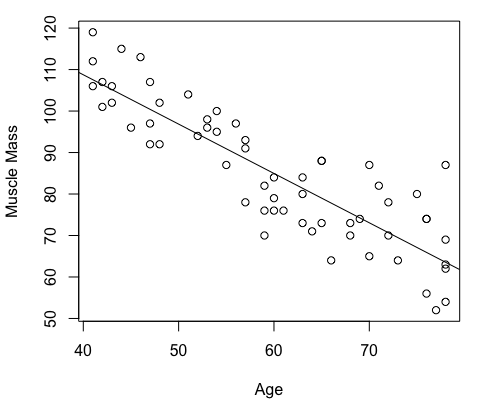
\includegraphics[width=.7\linewidth]{27a.png}
	\end{figure}
	This function appears to give a good fit and the plot supports the anticipation.
	
	\item [b.]
	\begin{enumerate}
		\item [(1)]
		A point estimate of the difference in the mean muscle mass for women differing in age by one year is $\hat{\beta}_1 = -1.19$.
		
		\item [(2)]
		A point estimate of the mean muscle mass for women aged $X=60$ years is $-1.19(60) + 156.35 = 84.95$.
		
		\item [(3)]
		The value of the residual for the eighth case, where $X=41$ and $Y=112$ is $e_8 = Y_8 - \hat{Y}_8 = 112 - [-1.19(41) + 156.35] = 4.44$.
		
		\item [(4)]
		A point estimate of $\sigma^2$ is $\hat{\sigma}^2 = \frac{RSS}{n-2} = \frac{3874.4}{58} = 66.8$.
		\lstinputlisting{27b4.txt}
	\end{enumerate}
\end{enumerate}

\subsection*{Ex 1.28}
\begin{enumerate}
	\item [a.]
	The estimated regression function is $\hat{Y} = -170.6x + 20517.6$.
	\lstinputlisting{28a.txt}
	The plot of the function and the data is shown below:
	\begin{figure}[H]
		\centering
		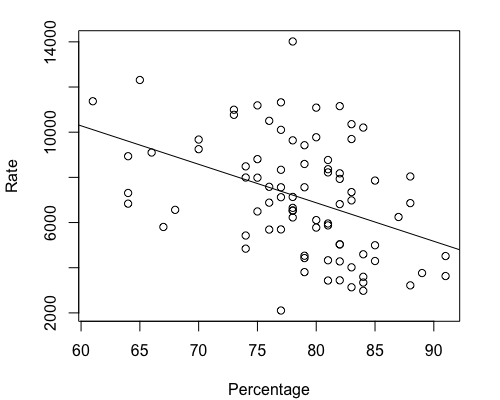
\includegraphics[width=.6\linewidth]{28a.png}
	\end{figure}
	This function generally gives not a very good but acceptable fit since the correlation between $X$ and $Y$ here is not that strong.
	
	\item [b.]
	\begin{enumerate}
		\item [(1)]
		A point estimate of the difference in the mean crime rate for two countries whose high-school graduation rates differ by one percentage point is $\hat{\beta}_1 = -170.6$.
		
		\item [(2)]
		A point estimate of the mean crime rate last year in countries with high school graduation percentage $X=80$ is $-170.6(80) + 20517.6 = 6869.6$.
		
		\item [(3)]
		A point estimate of $\epsilon_{10}$, where $X=82$ and $Y=7932$ is $e_{10} = Y_{10} - \hat{Y}_{10} = 7932 - [-170.6(82) + 20517.6] = 1403.6$.
		
		\item [(4)]
		A point estimate of $\sigma^2$ is $\hat{\sigma}^2 = \frac{RSS}{n-2} = \frac{455273165}{82} = 5552112$.
		\lstinputlisting{28b4.txt}
	\end{enumerate}
\end{enumerate}

\subsection*{Ex 1.39}
\begin{enumerate}
	\item [a.]
	Let $Y_{i,1}$ and $Y_{i,2}$ be the observations on $Y$ whose mean is $\bar{Y}_i, i=1,2,3$. For the six points,
	\begin{align*}
		\hat{\beta}_1^* 
		&= \frac{S_{xy}^*}{S_{xx}^*}\\
		&= \frac{\sum_{i=1}^{3} (x_i - \bar{x})(y_{i,1}-\bar{y}) + (x_i - \bar{x})(y_{i,2}-\bar{y}) }{\sum_{i=1}^{3} (x_i - \bar{x}) + (x_i - \bar{x})}\\
		&= \frac{\sum_{i=1}^{3} 2(x_i - \bar{x})(\frac{y_{i,1} + y_{i,2}}{2}-\bar{y}) }{2\sum_{i=1}^{3}(x_i - \bar{x})}\\
		&= \frac{\sum_{i=1}^{3} (x_i - \bar{x})(\bar{Y}_i-\bar{y})}{\sum_{i=1}^{3}(x_i - \bar{x})}\\
		&= \frac{S_{xy}}{S_{xx}}
	\end{align*}
	where $S_{xy}$ and $S_{xx}$ are for three points. So, $\hat{\beta}_1$ is the same for three-point case and six-point case. Since the mean values $\bar{x}$ and $\bar{y}$ are both the same in two cases, $\hat{\beta}_0 = \bar{y} - \hat{\beta}_1 \bar{x}$ is also the same. Therefore, the least squares regression lines are identical.
	
	\item [b.]
	Since $RSS = S_{yy} - \frac{S_{xy}^2}{S_{xx}}$ and $\hat{\sigma}^2 = \frac{RSS}{n-2}$, we can directly calculate the estimate of $\sigma^2$ without fitting a regression line.
\end{enumerate}

\subsection*{Ex 1.42}
\begin{enumerate}
	\item [a.]
	\[
	L(\beta_1) = \prod_{i=1}^{n} f(y_i | \beta_1, \sigma^2) = \pa{\frac{1}{4\sqrt{2\pi}}}^6 \exp\pa{-\frac{1}{32} \sum_{i=1}^{n} (y_i - \beta_1 x_i)^2}
	\]
	
	\item [b.]
	$L(17) = 9.45133\times 10^{-30}, L(18) = 2.64904\times 10^{-7}, L(19) = 3.04729\times 10^{-37}$. The likelihood function is largest at $\beta_1 = 18$.
	
	\item [c.]
	$b_1 = \sum_{i=1}^{6} X_i Y_i / \sum_{i=1}^{6} X_i^2 = 17.9285$. The result in part (b) is close to the estimate.
	
	\item [d.]
	The plot for the likelihood function is shown below.
	\begin{figure}[H]
		\centering
		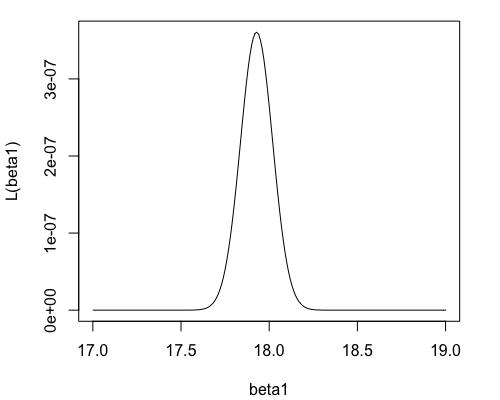
\includegraphics[width=.5\linewidth]{42d.png}
	\end{figure}
	The point where the likelihood function is maximized corresponds to what's found in part (c).
\end{enumerate}

{\large\bf Show that $\ds \sum_{i=1}^{n} e_i x_i = 0$ and $\ds \sum_{i=1}^{n} e_i = 0$.}
\begin{align*}
	\sum_{i=1}^{n} e_i x_i
	&= \sum_{i=1}^{n} x_i[y_i - (\bar{y} - \hat{\beta}_1 \bar{x}) - \hat{\beta}_1 x_i]\\
	&= \sum_{i=1}^{n} x_i y_i - \bar{y}\sum_{i=1}^{n}x_i + \hat{\beta}_1 \bar{x} \sum_{i=1}^{n} x_i - \hat{\beta}_1 \sum_{i=1}^{n} x_i^2\\
	&= \sum_{i=1}^{n} x_i y_i - n\bar{x}\bar{y} + \frac{\sum_{i=1}^{n} x_i y_i - n\bar{x}\bar{y}}{\sum_{i=1}^{n} x_i^2 - n\bar{x}^2}\pa{n\bar{x}^2 + \sum_{i=1}^{n} x_i^2}\\
	&= \sum_{i=1}^{n} x_i y_i - n\bar{x}\bar{y} - \pa{\sum_{i=1}^{n} x_i y_i - n\bar{x}\bar{y}}\\
	&= 0\\
	\sum_{i=1}^{n} e_i
	&= \sum_{i=1}^{n} [y_i - (\bar{y} - \hat{\beta}_1 \bar{x}) - \hat{\beta}_1 x_i]\\
	&= \sum_{i=1}^{n} y_i - n\bar{y} + \hat{\beta}_1 n\bar{x} - \hat{\beta}_1 \sum_{i=1}^{n} x_i\\
	&= n\bar{y} - n\bar{y} + \hat{\beta}_1 n\bar{x} - \hat{\beta}_1 n\bar{x}\\
	&= 0
\end{align*}

{\large\bf Show that $\hat{\beta}_1 \sim N(\beta_1, \sigma^2/\sum_{i=1}^{n} (x_i - \bar{x})^2)$.}
\[
\hat{\beta}_1 = \frac{\sum_{i=1}^{n} (x_i - \bar{x})(y_i - \bar{y})}{S_{xx}} = \frac{\sum_{i=1}^{n} (x_i - \bar{x}y_i)}{S_{xx}} - \frac{\bar{y}\sum_{i=1}^{n} (x_i - \bar{x})}{S_{xx}} = \frac{\sum_{i=1}^{n} (x_i-\bar{x})y_i}{S_{xx}}
\]
Let $k_i = \frac{x_i - \bar{x}}{S_{xx}}, i=1,\dots,n$, then $\hat{\beta}_1 = \sum_{i=1}^{n} k_i y_i$. Since $k_i$ possess the properties:
\begin{align*}
	\sum_{i=1}^{n} k_i &= 0\\
	\sum_{i=1}^{n} k_i x_i &= 1\\
	\sum_{i=1}^{n} k_i^2 &= \frac{1}{S_{xx}}
\end{align*}
we can derive that
\begin{align*}
	E(\hat{\beta}_1) &= E\pa{\sum_{i=1}^{n} k_i Y_i} = \sum_{i=1}^{n} k_i E(Y_i) = \sum_{i=1}^{n} k_i (\beta_0 + \beta_1 x_i) = \beta_0 \sum_{i=1}^{n} k_i + \beta_1 \sum_{i=1}^{n} k_i x_i = \beta_1\\
	var(\hat{\beta}_1) &= var\pa{\sum_{i=1}^{n} k_i Y_i} = \sum_{i=1}^{n} k_i^2 var(Y_i) = \sum_{i=1}^{n} k_i^2\sigma^2 = \frac{\sigma^2}{S_{xx}}
\end{align*}
Since $Y_i$'s are assumed to be normally distributed with mean $\mu_i$ and variance $\sigma_i^2$ , the moment-generating function is given by
\[
m_{Y_i}(t) = \exp\pa{\mu_i t + \frac{\sigma_i^2 t^2}{2}}
\]
Then
\begin{align*}
	m_{\hat{\beta}_1}(t)
	&= \prod_{i=1}^n m_{k_i Y_i}(t)\\ \ds
	&= \prod_{i=1}^n \exp\pa{\mu_i k_i t + \frac{k_i^2 \sigma_i^2 t^2}{2}}\\
	&= \exp\pa{t\sum_{i=1}^{n} k_i \mu_i + \frac{t^2}{2} \sum_{i=1}^{n} k_i^2 \sigma_i^2}
\end{align*}
Therefore, $\hat{\beta}_1$ is also normally distributed. Thus,
\[
\hat{\beta}_1 \sim N\pa{\beta_1, \sigma^2/\sum_{i=1}^{n} (x_i - \bar{x})^2}
\]

\end{document}
